\begin{exercise}{Confinement dans un puits fini}{2}{Spé}
{Quantique}{lelay}

On considère une particule dans le potentiel suivant : Il s'agit d'un puits fini de hauteur $V$, de largeur $L$, centré en 0. On ne considère dans cet exercices que le cas d'une particule d'énergie $E < V$.

\begin{center}
    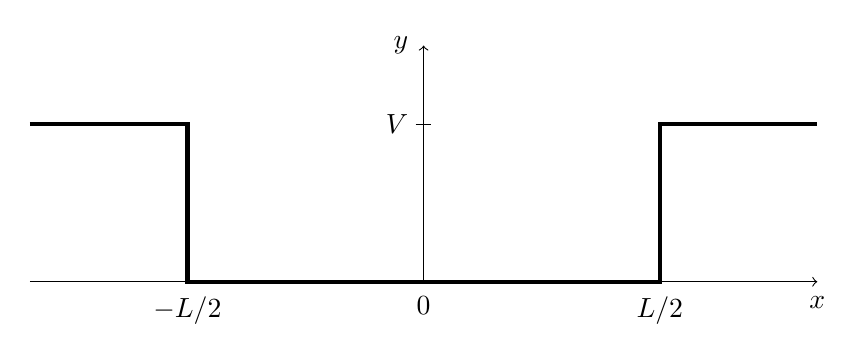
\begin{tikzpicture}
    
    \draw[->] (-5, 0) -- (5, 0);
    \draw (5,0) node[below=2pt] {$x$};
    \draw (0,0) node[below=2pt] {$0$};
    \draw (-3,0) node[below=2pt] {$-L/2$};
    \draw (3,0) node[below=2pt] {$L/2$};
    
    \draw[->] (0, 0) -- (0, 3);
    \draw (0,3) node[left=2pt] {$y$};
    \draw[] (-0.1, 2) -- (0.1, 2);
    \draw (0,2) node[left=2pt] {$V$};
    
    
    \draw[ultra thick] (-5, 2) -- (-3, 2) -- (-3, 0) -- (3 , 0) -- (3, 2) -- (5, 2);
    
    \end{tikzpicture}
\end{center}

\begin{questions}
    \questioncours Quantification de l'énergie dans le cas d'une particule dans un puits de potentiel infini.
    \question Justifier qu'une particule d'énergie $E< V$ sera confinée dans le puits. L'énergie $E$ peut-elle être quelconque ?
    \question Estimer l'incertitude $\Delta x$ sur la position de cette particule.
    \question Quelles sont les énergies $E$ autorisées pour une particule ? Quelle(s) différence(s) avec le cas du puits infini ?
    \question Représenter les fonctions d'ondes pour les première énergie autorisées (en supposant qu'elles existent).
\end{questions}

\end{exercise}

\begin{solution}

\begin{questions}
    \questioncours Puits infini : $E = \hbar^2k^2/2m$ mais $L = n \lambda/2$ soit $k = n \pi/L$
    \question Énergie plus petite que le potentiel à l'infini donc état lié. Pour un état lié en quantique l'énergie est quantifiée.
    \question Naivement $\Delta x \sim L/2$ mais il y a dépassement sur une longueur caractéristique $\delta = \hbar/\sqrt{2m(V-E)}$ des deux côtés, d'où $\Delta x \sim L/2 + \delta$
    \question Il faut séparer les modes symétriques et antisymétriques (qui sont linéairement indépendants). Dans la limite $V \gg E$, les modes symétriques ont $k = \pi/L + 2n\pi/L$, $n\in \mathbb{N}$ et les modes antisymétriques $k = 2m\pi/L$, $m\in \mathbb{N}^*$. On retrouve bien les modes de puits infini. En réalité les $k$ sont toujours un peu plus faible que dans le cas infini : la longueur d'onde est plus grande parce que la taille effective du puits est augmentée.
    \question Sym, antisym, sym, avec débordement et jonctions smooth.
\end{questions}
\end{solution}